\documentclass[12pt, titlepage]{article}

\usepackage{booktabs}
\usepackage{float}
\usepackage{tabularx}
\usepackage{longtable}
\usepackage{hyperref}
\hypersetup{
    colorlinks,
    citecolor=black,
    filecolor=black,
    linkcolor=red,
    urlcolor=blue
}
\usepackage[round]{natbib}
\usepackage{graphicx}

%% Comments

\usepackage{color}

\newif\ifcomments\commentstrue %displays comments
%\newif\ifcomments\commentsfalse %so that comments do not display

\ifcomments
\newcommand{\authornote}[3]{\textcolor{#1}{[#3 ---#2]}}
\newcommand{\todo}[1]{\textcolor{red}{[TODO: #1]}}
\else
\newcommand{\authornote}[3]{}
\newcommand{\todo}[1]{}
\fi

\newcommand{\wss}[1]{\authornote{blue}{SS}{#1}} 
\newcommand{\plt}[1]{\authornote{magenta}{TPLT}{#1}} %For explanation of the template
\newcommand{\an}[1]{\authornote{cyan}{Author}{#1}}

%% Common Parts

\newcommand{\progname}{ProgName} % PUT YOUR PROGRAM NAME HERE
\newcommand{\authname}{Team \#, Team Name
\\ Student 1 name
\\ Student 2 name
\\ Student 3 name
\\ Student 4 name} % AUTHOR NAMES                  

\usepackage{hyperref}
    \hypersetup{colorlinks=true, linkcolor=blue, citecolor=blue, filecolor=blue,
                urlcolor=blue, unicode=false}
    \urlstyle{same}
                                


\begin{document}

\title{Verification and Validation Report: \progname} 
\author{\authname}
\date{\today}
	
\maketitle

\pagenumbering{roman}

\section{Revision History}

\begin{tabularx}{\textwidth}{p{3cm}p{2cm}X}
\toprule {\bf Date} & {\bf Version} & {\bf Notes}\\
\midrule
March 6, 2023 & 1.0 & Initial Vesrion\\
\bottomrule
\end{tabularx}

~\newpage

\section{Symbols, Abbreviations and Acronyms}

\renewcommand{\arraystretch}{1.2}

\begin{table}[H]
\begin{center}
\begin{tabular}{|p{3cm}|p{9cm}|}
\hline
  \textbf{Symbol} & \textbf{Description}\\
  \hline
  Data Structures and Algorithms & A topic of study for Computer Scientists.\\
  \hline
  CodeChamp & The system being built and tested.\\
  \hline
  Angular & A web framework for building web applications.\\
  \hline
  API & Abbreviation for Application Program Interface.\\
  \hline
  DSA & Abbreviation for Data Structures and Algorithms.\\
  \hline
  CI & Abbreviation for Continuous Integration.\\
  \hline
  SRS & Abbreviation for Software Requirements Specification.\\
  \hline
  MIS & Abbreviation for Module Interface Specification.\\
  \hline
  MG & Abbreviation for Module Guide.\\
  \hline
  Mocha & A JavaScript testing framework.\\
  \hline
  Jasmine &  A JavaScript testing framework.\\
  \hline
  GitHub & A service for software development and version control.\\
  \hline
  GitHub Actions & A CI system integrated with GitHub.\\
  \hline
\end{tabular}
\end{center}
\caption{Symbols, Abbreviations and Acronyms}            

\end{table}

\newpage

\tableofcontents

\listoftables %if appropriate

\listoffigures %if appropriate

\newpage

\pagenumbering{arabic}

\section{Introduction}
This document describes the verification \& validation effort for the CodeChamp system. Other relevant documentation is listed below:
\begin{enumerate}
    \item \href{https://github.com/Tamas-Leung/CodeChamp/blob/main/docs/VnVPlan}{Validation \& Verification Plan} 
    \item \href{https://github.com/Tamas-Leung/CodeChamp/tree/main/docs/DevelopmentPlan}{Development Plan}
    \item \href{https://github.com/Tamas-Leung/CodeChamp/tree/main/docs/SRS}{System Requirements Specification} 
    \item \href{https://github.com/Tamas-Leung/CodeChamp/blob/main/docs/HazardAnalysis/HazardAnalysis.md}{Hazard Analysis}
    \item \href{https://github.com/Tamas-Leung/CodeChamp/blob/main/docs/Design/SystDesign/SystemDesign.pdf}{Design Documentation}
    
\end{enumerate}

\section{Purpose}

This document is written to describe the steps taken to verify \& validate the  requirements and the implementation for the CodeChamp system. Primarily, it describes the functional requirements evaluated in accordance to the Validation \& Verification plan. Moreover, it reports the results of the testing in regards to non-functional requirement. It  also delves deeper into the validation and verification of two non-functional requirements: usability and security, which are of particular importance to the CodeChamp system. Additionally, unit testing done by the testers is summarized, as well as the ways in which automated testing tools were leveraged. Finally, the changes due to testing are summarized and justified and the tractability between the requirements, modules and tests are given. 

\section{Functional Requirements Evaluation}
The functional requirements evaluation is summarized by Table \ref{tab:functional Tests Requirements}:

\begin{longtable}{| p{2.5cm} | p{11cm} |}
    \hline
    Test Case ID & Testing Result\\
    \hline
    TC-MM-1 & Passed, tester found response time to be well below the maximum response time.\\
    \hline
    TC-MM-2 & Passed, tester was able to join a existing lobby with the correct lobby code shared by friends. \\ 
     \hline
    TC-MM-3 & Passed, tester was able to create a lobby using the create button in the home page.\\
     \hline
    TC-IG-1 & Passed, testers were able to complete a match by winning or losing match.\\
     \hline
    TC-IG-2 & Passed, input given was able to compile a solution.\\
     \hline
    TC-PM-1 & Passed, tester was able to add new problems using admin account.\\
     \hline
    TC-PM-2 & Passed, tester was able to modify problems using admin account.\\
     \hline
    TC-PM-3 & Passed, tester was able to delete problems using admin account.\\
     \hline
    TC-PV-1 & Passed, profile was able to display wins and losses.\\
     \hline
    TC-PV-2 & Passed, profile was able to display match history.\\
     \hline
    TC-LB-1 & Passed, tester was able to see data of leaderboard tests.\\
     \hline
    % \end{tabularx}
    \caption{Functional Test Cases and Requirements}
    \label{tab:functional Tests Requirements}
\end{longtable}


\section{Non-functional Requirements Evaluation}
The non-functional requirements evaluation is summarized by Table \ref{tab:non-functional Tests Requirements}:

\begin{longtable}{| p{2.5cm} | p{11cm} |}
    \hline
    Test Case ID & Testing Result\\
    \hline
    TC-LF-1 & Passed after Changes, information below in Usability section \ref{sec:usabilty}.\\
    \hline
    TC-LF-2 & Passed, all screen sizes worked as expected.\\
    \hline
    TC-P-1 & Passed, Chrome Dev Tools showed response time less than the maximum response time when an action was performed.\\
    \hline
    TC-P-2 & Passed, Chrome Dev Tools showed response time less than the maximum compile time when a compilation was performed. \\
     \hline
    TC-OE-1 & Passed, the program was tested on devices on multiple OS(mac, windows) and in combination with browsers(Google Chrome, Firefox and Safari).\\
     \hline
    TC-S-1 & Passed after changes, testers were able to call functions for other users as long as they had their user id and the game id they were currently in. Changes were made to fix this through authentication checking. Further discussed in \ref{sec:changes}.\\
     \hline
    TC-S-2 & Passed after changes, the leaderboard page displays user emails.\\
     \hline
    TC-C-1 & Passed, the game did not have any cultural references.\\
     \hline
    TC-L-2 & Passed, the repository was protected by the GNU license.\\
     \hline
    % \end{tabularx}
    \caption{Non-Functional Test Cases and Requirements}
    \label{tab:non-functional Tests Requirements}
\end{longtable}

\subsection{Usability}\label{sec:usabilty}

In addition to the non-functional tests for usability, a semi-structured interview was conducted with a total of eight users in the target demographic. To achieve this, a CodeChamp lobby was setup with the users. This included current Computer Science and Software Engineering students, as well as current Software Engineering professionals. After finishing a game, each user was asked several questions. Rough notes from the interviews can be found in the Appendix, under section \ref{roughnotes}. The questions, interview structure and results are summarized below:

\begin{itemize}
    \item From 1 - 10, How easy was the interface to navigate? 
    1 being un-navigatable, 10 being no issues navigating.

    If users answered less than 8, we would follow up and ask for feedback. The result for this question were that all users said the interface was simple and all ratings were 9 or above. Figure \ref{FigUH-1} below summarizes the results for this question:

    \begin{figure}[H]
    \centering
    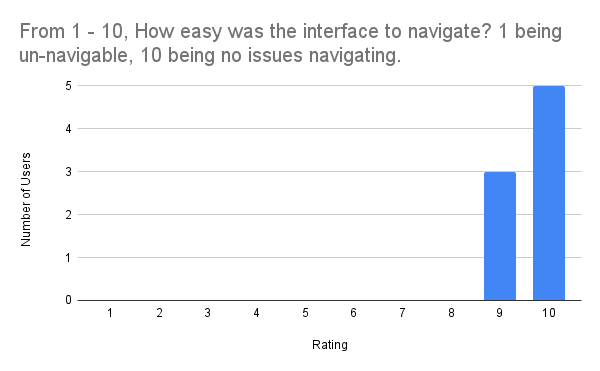
\includegraphics[width=1\textwidth]{question1chart.png}
    
    \caption{Graph depicting results for interface navigation usability}
    
    \label{FigUH-1}
    \end{figure}

    \item From 1 - 10, How consistent was the visual theming of the website? 1 being not consistent at all, 10 being super consistent. 

    If users answered less than 8, we would follow up and ask for feedback. The result for this question were that most users rated 7 or above. Users who said 7 and 8 mentioned that the game screen and login screen had a different colour scheme than the rest of the website. Figure \ref{FigUH-2} below summarizes the results for this question:

    \begin{figure}[H]
    \centering
    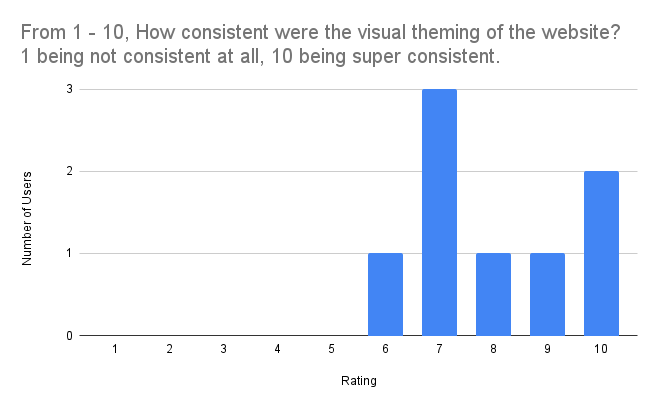
\includegraphics[width=1\textwidth]{question2chart.png}
    
    \caption{Graph depicting results for visual theming consistency usability}
    
    \label{FigUH-2}
    \end{figure}

    \item For testing whether users wanted the copy code button to copy the whole URL or just the game id. Our team did A/B testing where half the users were tested on copying the URL then trying copying the game id and vice versa for the other group. Our testing found that most players preferred sending the whole URL. Figure \ref{FigUH-3} below summarizes the results for this question:
    \begin{figure}[H]
    \centering
    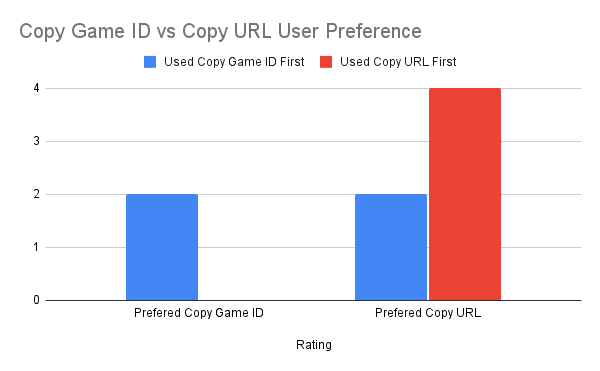
\includegraphics[width=1\textwidth]{question3chart.png}
    
    \caption{Graph depicting results for copying url versus copying game id}
    
    \label{FigUH-3}
    \end{figure}

    \item A asked for if users felt that any feature was missing from the game. The most common feature missing was stats. When asked about what information the profile page should give. The most common ask was for the difficulty of problems solved as well as calculating their win rate.

    \item When asked on what additional languages were preferred to be used. The most common response given was Python. Figure \ref{FigUH-4} below summarizes the results for this question:

    \begin{figure}[H]
    \centering
    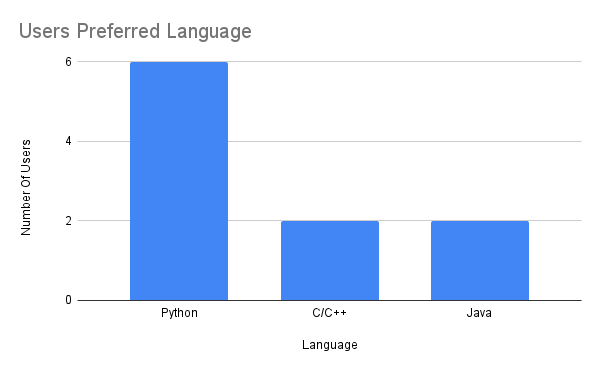
\includegraphics[width=1\textwidth]{question4chart.png}
    
    \caption{Graph depicting results for most preferred language to use for data structures and algorithms}
    
    \label{FigUH-4}
    \end{figure}
    
\end{itemize}

\subsection{Security}\label{sec:security}
A critical part of the CodeChamp system involves compiling and executing user code, which can be potentially destructive to the system's security. To test this, several scripts were written to enact malicious / dangerous submissions and fed into the CodeChamp Judge system. Afterwards, the testers ensured that the system was able to prevent 100\% of the scenarios from negatively affecting or compromising the CodeChamp system.

Table \ref{tab:Security} below summarizes the scenarios which were considered as part of the security evaluation:

\begin{longtable}{| p{3cm} | p{5.5cm} | p{5cm} |}
    \hline
    Security Concern & Scenario & Result\\
    \hline
    Accessing the CodeChamp server's file system & Code which tries to write a file to the file system was submitted. & No file was written to the CodeChamp file system, as it was only written to the local container which was killed afterwards.\\
    \hline
    Accessing the CodeChamp server's file system & Code which tries to remove a file from the file system was submitted. & No file was removed from the CodeChamp file system.\\
    \hline
    Hogging server resources due to non-terminating code. & Code including an infinite loop was submitted to a problem with a 3 second time limit. & The Judge system returned a TLE (Time-Limit Exceeded) code. The container running the code was killed. \\
    \hline
    Hogging server resources due to  unnecessarily large memory usage. & Code which initializes a large array was submitted to a problem with a 64 MegaByte memory limit. & The Judge system returned a MLE (Memory-Limit Exceeded) code. The container running the code was killed. \\
     \hline
     Potential code Injections, cheating / hacking concerns & Code which makes an HTTP request was submitted. & The Judge system returned a Code Error, which resulted from an unhandled exception due to the failing network call. The container running the code was killed. \\
     \hline
    \caption{Security Scenarios Considered for CodeChamp Judge System}
    \label{tab:Security}
\end{longtable}

\section{Unit Testing}

Unit testing was done for all applicable modules. For back-end modules, Mocha was used as the unit testing framework. For front-end modules, Jasmine was used. Additionally, these tests were automated as described in Section \ref{sec:auto}. In particular, for back-end testing, all API endpoints were tested. This covered operations of creating, reading, updating, and deleting data. The data we used to verify these operations were mocked data that was used by a mock database for the purposes of testing. For front-end testing, we tested components for each page. This involved testing the usability and functionality of menus, buttons, interactions, events and other GUI elements visible to the user using a Chrome runner.


\section{Changes Due to Testing}\label{sec:changes}

% \wss{This section should highlight how feedback from the users and from 
% the supervisor (when one exists) shaped the final product.  In particular 
% the feedback from the Rev 0 demo to the supervisor (or to potential users) 
% should be highlighted.}

After receiving feedback from the Rev 0 demo, we changed the mechanism for copying a lobby's unique code. What we initially had was copying the code itself, but we changed the text that would be copied to the URL of the lobby. This way, instead of entering the code to join a lobby, the URL can be used to join the lobby, reducing the number of clicks the user has to go through. This was A/B tested as previously discussed in the usability section, with the majority of users preferring this option.

Feedback from users also initiated the change of statistics that will be shown to the users when viewing their profile. Initially we gave information regarding the win, loss, and the questions solved in each game. According to our testing, users would like to know the number of problems of each difficulty they have solved. Now we have the addition of the types of problems solved in terms of difficulty. This allows users to track their success against easy, medium, and hard level questions. Alongside the total wins and losses for a player, we have added the respective ratio so they do not have to calculate it themselves.

More programming languages are supported to allow individuals with proficiency in different programming languages to compete on the platform. After a survey with the users indicating which languages we should support, Python was voted the highest among other languages like C++, Java, and C. As a result, we have added support for the Python language to be used on the CodeChamp platform. 

With the user testing for the look and feel non-functional requirement (TC-LF-1) 2 users found that the system's lack of consistency in the design. This included the design of the game page as well as the login page. With this feedback, game and login pages were redesigned and implemented to be consistent with the rest of the application.

After user acceptance testing, some users brought up that they were uncomfortable with emails being displayed in the leaderboards. Additionally, this violates a security  requirement of storing and displaying only the necessary data (TC-S-2). As this is a private data point of the user, it should not be displayed as it may compromise the user's Google and other accounts associated. Due to this, the email display was changed to the user's username. 

The current implementation uses a player's ID as their email. Thus, submissions from users that are not actually involved in a game can be allowed if a malicious user discovers this, and is able to somehow reverse-engineer or discover the game ID for a particular game. Due to this an authentication middleware is applied to the backend for communication from clients to fulfil the requirement of user authenticity (UC-S-1). 

\section{Automated Testing}\label{sec:auto}

GitHub Actions were used to automatically test new pull requests using Mocha and Jasmine, which were used to test the back-end and front-end, respectively. Additionally, linting and formatting rules were written using ESLint and Prettier using the \href{https://github.com/airbnb/javascript}{Airbnb style guide} and the \href{https://angular.io/guide/styleguide}{official Angular style guide} for reference. The code-base was checked against these rules using GitHub actions on every pull request as well.

\section{Trace to Requirements}
\begin{longtable}{| p{2.5cm} | p{3cm} | p{8cm}| }
    \hline
    Test Case ID & Requirement ID & Requirement Description\\
    \hline
    TC-MM-1 & FR.1 & Should join a random match.\\
    \hline
    TC-MM-2 & FR.24 & Should join an existing page with a code. \\
     \hline
    TC-MM-3 & FR.23 & Should create a match. \\
     \hline
    TC-IG-1 & FR.2, FR.3, FR.4, FR.5, FR.8, FR.9, FR.10, FR.11 & Should complete a match. \\
     \hline
    TC-IG-2 & FR.6, FR.7, FR.20, FR.21 & Should compile solutions from input.\\
     \hline
    TC-PM-1 & FR.12, FR.13, FR.22, NFR.10 & Should be able to add new problems (admin).\\
     \hline
    TC-PM-2 & FR.12, FR.13, FR.22, NFR.10 & Should be able to modify problems (admin).\\
     \hline
    TC-PM-3 & FR.12, FR.13, FR.22, NFR.10 & Should be able to delete problems (admin).\\
     \hline
    % TC-LS-1 & FR.17 & New users can sign up. \\
    %  \hline
    % TC-LS-2 & FR.18  & Existing users can log in. \\
    %  \hline
    % TC-LS-3 & FR.19  & Login with invalid information is rejected and a error message is displayed. \\
     % \hline
    TC-PV-1 & FR.26 & Profile should view win percentage.\\
     \hline
    TC-PV-2 & FR.25, FR.27, FR.28  & Profile should view match history.\\
     \hline
    TC-LB-1 & FR.29 & Leaderboard view should show the players sorted by their scores.\\
     \hline
    TC-LF-1 & NFR.1, NFR.2, NFR.3, NFR.4, NFR.5 & Ease of navigation.\\
    \hline
    TC-LF-2 & NFR.1, NFR.3  & Compatibility among devices.\\
    \hline
     TC-P-1 & NFR.6 & Performance of user actions.\\
    \hline
    TC-P-2 & NFR.7 & Performance of user solution compilation.\\
     \hline
    TC-OE-1 & NFR.9 & Should run on any modern browser on any device. \\
     \hline
    TC-S-1 & NFR.11, NFR.12 & Only requests from authenticated users should be accepted. \\
     \hline
    TC-S-2 & NFR.11 & Only minimal data about a user should be stored.\\
     \hline
    TC-C-1 & NFR.13 & Content of the system should not contain any cultural references.\\
     \hline
    TC-L-2 & NFR.14 & System should be protected by GNU License.\\
     \hline
    % \end{tabularx}
    \caption{Traceability Table for Test Cases and Requirements}
    \label{tab:trace}
\end{longtable}

\section{Trace to Modules}
\begin{longtable}{| p{2.5cm} | p{5cm} | p{6cm}| }
    \hline
    Test Case ID & Module ID(s) & Test Case Description\\
    \hline
    TC-MM-1 & HomePage, LobbyPage, LobbyService, WebSocketService, GameHandler & Should join a random match.\\
    \hline
    TC-MM-2 &  HomePage, LobbyPage, LobbyService, WebSocketService, GameHandler & Should join an existing page with a code. \\
     \hline
    TC-MM-3 &  HomePage, LobbyPage, LobbyService, WebSocketService, GameHandler & Should create a match. \\
     \hline
    TC-IG-1 & GamePage, ProblemsService, SubmissionService, UserService, GameHandler & Should complete a match. \\
     \hline
    TC-IG-2 & GamePage, ProblemsService, SubmissionService, GameHandler & Should compile solutions from input.\\
     \hline
    TC-PM-1 & ProblemsService & Should be able to add new problems (admin).\\
     \hline
    TC-PM-2 & ProblemsService & Should be able to modify problems (admin).\\
     \hline
    TC-PM-3 & ProblemsService & Should be able to delete problems (admin).\\
     \hline
    TC-PV-1 & ProfilePage, UserService & Profile should view win percentage.\\
     \hline
    TC-PV-2 &  ProfilePage, UserService & Profile should view match history.\\
     \hline
    TC-LB-1 & LeaderboardPage, UserService & Leaderboard view should show the players sorted by their scores.\\
     \hline
    TC-LF-1 & All page modules & Ease of navigation.\\
    \hline
    TC-LF-2 & All page modules  & Compatibility among devices.\\
    \hline
     TC-P-1 & All modules & Performance of user actions.\\
    \hline
    TC-P-2 & SubmissionService & Performance of user solution compilation.\\
     \hline
    TC-OE-1 & All page modules & Should run on any modern browser on any device. \\
     \hline
    TC-S-1 & LoginPage, AuthService & Only requests from authenticated users should be accepted. \\
     \hline
    TC-S-2 & AuthService, UserService, SubmissionService & Only minimal data about a user should be stored.\\
     \hline
    TC-C-1 &  All page modules & Content of the system should not contain any cultural references.\\
     \hline
    TC-L-2 & N/A & System should be protected by GNU License.\\
     \hline
    % \end{tabularx}
    \caption{Traceability Table for Test Cases and Modules}
    \label{tab:trace}
\end{longtable}


\bibliographystyle{plainnat}
\bibliography{../../refs/References}

\newpage{}
\section*{Appendix}

\subsection{Reflection}
The information in this section will be used to evaluate the team members on the
graduate attribute of Reflection.  Please answer the following question:

\begin{enumerate}
  \item In what ways was the Verification and Validation (VnV) Plan different
  from the activities that were actually conducted for VnV?  If there were
  differences, what changes required the modification in the plan?  Why did
  these changes occur?  Would you be able to anticipate these changes in future
  projects?  If there weren't any differences, how was your team able to clearly
  predict a feasible amount of effort and the right tasks needed to build the
  evidence that demonstrates the required quality?  (It is expected that most
  teams will have had to deviate from their original VnV Plan.)
  
  
\end{enumerate}


  The biggest change from the VnV plan was the addition of user acceptance testing. As our platform is user-centric, with the goal of teaching users, it is essential that we measure the user's experience to understand if it fulfills their needs. This involved adding interview questions, as well as reaching out to target demographic members in order to setup a testing session. With the bigger emphasis on usability testing through user acceptance testing, there was less time to spend on automated testing. This resulted in a deviation from the original VnV plan for functional testing, which included automated end-to-end (E2E) tests for the majority of the requirements. While E2E tests are crucial to catching regressions in a constantly evolving system, it was determined to be a sub-optimal use of the team's testing budget at this stage for a multitude of reasons. Primarily, many of the requirements and modules that would be tested using E2E tests are also covered by unit tests. Additionally, the majority of the functional tests were also tested by other users during the user acceptance sessions, as well as by the developers of the platform and the instructors during development and demonstrations. Finally, automating the E2E tests to run using GitHub actions is significantly more time consuming than other types of tests, as it requires to sandbox the entire platform to be run (i.e. the server, client, database, browser). For these reasons, there was enough confidence to modify this section of the VnV plan. In the future, it would be beneficial to consider a broader range of testing techniques from an earlier stage, as the original VnV plan was too focused on functional testing and thus did not consider other aspects such as the user experience. Therefore, with better scoping, we could have anticipated these changes by analyzing the aspects which the end-user will interact with the most, and dividing the testing budget to cover the most crucial aspects.
  
\subsection{Usability Interview Rough Notes}\label{roughnotes}
Questions:
\begin{enumerate}
    \item From 1 - 10, How easy was the interface to navigate? 1 being un-navigable, 10 being no issues navigating.
    \item From 1 - 10, How consistent were the visual theming of the website? 1 being not consistent at all, 10 being super consistent. 
    \item Do you prefer the copy code button to copy the game id or the full url?
    \item What language do you prefer to learn data structures and algorithms for?
    \item What feature is missing from the website that you would like implemented?
\end{enumerate}


\begin{enumerate}
    \item User 1 - Man, Third year Computer Science student
    \begin{itemize}
        \item Q1: 10
        \item Q2: 7. The overall theme looks great, however the game screen looks like a different part of the website.
        \item Q3: Tested copy game id first. Preferred copying the full url.
        \item Q4: Python
        \item Q5: Nothing
    \end{itemize}
    \item User 2 - Man, Fourth year Software Engineering student
    \begin{itemize}
        \item Q1: 9
        \item Q2: 10
        \item Q3: Tested copy full url first. Preferred copying the full url
        \item Q4: Java
        \item Q5: The timer should vary for each problem based on the difficulty. The timer should count faster when people have finished, similar to a racing game. The leaderboard should not display email, only username.
    \end{itemize}
    \item User 3 - Man, Fourth year Software Engineering student
    \begin{itemize}
        \item Q1: 10
        \item Q2: 8, Felt dark colors on game page did not match color scheme
        \item Q3: Tested copy game id first. Preferred Game ID.
        \item Q4: C++
        \item Q5: Addition of more stats, wanted win rate. The Leaderboard should not have emails.
    \end{itemize}
    \item User 4 - Man, Industry Junior Software Developer
    \begin{itemize}
        \item Q1: 9
        \item Q2: 9
        \item Q3: Tested copy full url first. Preferred copying the full url
        \item Q4: Python
        \item Q5: Support for more languages. Problem hints.
    \end{itemize}
    \item User 5 - Woman, Fourth year Software Engineering student
    \begin{itemize}
        \item Q1: 9
        \item Q2: 7, half of the game page was light mode and the other was dark mode.
        \item Q3: Tested copy full url first. Preferred full url
        \item Q4: Python
        \item Q5: Performance stats per problem (which percentile is the solution)
    \end{itemize}
    \item User 6 - Woman, Fourth year Software Engineering student
    \begin{itemize}
        \item Q1: 10
        \item Q2: 10
        \item Q3: Tested copy game id first. Preferred copying the full url
        \item Q4: Python
        \item Q5: Detailed game history, ability to see opponents and their ranks or wins
    \end{itemize}
    \item User 7 - Man, Fourth year Computer Science student
    \begin{itemize} 
        \item Q1: 10
        \item Q2: 6, the game page does not match the rest of the website. 
        \item Q3: Tested copy game id first. Preferred game id
        \item Q4: C
        \item Q5: Ability to have a \% of people ready up (voting system) rather one person clicking ready
    \end{itemize}
    \item User 8 - Man, Fourth year Computer Science student
    \begin{itemize}
        \item Q1: 10
        \item Q2: 7 
        \item Q3: Tested copy full url first. Preferred full url
        \item Q4: Python
        \item Q5: Profile pages for all players, not just mine. Gives more visibility into the leaderboards.
    \end{itemize}
\end{enumerate}

\end{document}